% !TeX document-id = {49b9cd48-9a28-43d8-a1fd-030bc1e37b2e}
% % Konfiguration für Texstudio (Version > 2.9)
% !TeX program = pdflatex
%% !TeX TXS-program:compile = txs:///pdflatex/[--shell-escape]
% !BIB program = biber
% !TeX spellcheck = de_DE
% !TeX encoding = utf8
% !TeX root = Thesis.tex


\newcommand{\authorname}{Christof Pfannenm\"uller} 

% Header

\documentclass[
	a4paper,
	%oneside,
	twoside,
	12pt,
	numbers=noenddot,
	openright,	% Kapitel beginnt auf rechter Seite
	titlepage,	% Titelblatt auf eigener Seite
	bibliography=totoc,		% Literaturverzeichnis
	listof=totoc,	% Listen ins Inhaltsverzeichnis
	twoside,  % zweiseitig
]{scrbook}



\usepackage[english,ngerman,shorthands=off]{babel} % Deutsche Sprachanpassungen
\usepackage[T1]{fontenc}    % Silbentrennung bei Sonderzeichen
\usepackage[utf8]{inputenc} % Direkte Angabe von Umlauten im Dokument.
\usepackage{lmodern}					% Umlaute markierbar in PDF
\usepackage{textcomp}       % Zusätzliche Symbolzeichen
\usepackage{microtype}       % Optimierter Rand
\usepackage{amsmath}					% Formeln
\usepackage{graphicx}					% Graphiken einbinden
\usepackage{float}
\usepackage[german]{nomencl}
\usepackage[countmax]{subfloat}
\usepackage{wallpaper}

%\clubpenalty = 10000 % schliesst Schusterjungen aus
%\widowpenalty = 10000 % schliesst Hurenkinder aus


%eigene Packete
\usepackage{makeidx}
\makeindex
%eigene Packete ende

% Farben definieren für package listings 
\usepackage{color}
\definecolor{middlegray}{rgb}{0.5,0.5,0.5}
 \definecolor{lightgray}{rgb}{0.8,0.8,0.8}
 \definecolor{orange}{rgb}{0.8,0.3,0.3}
 \definecolor{yac}{rgb}{0.6,0.6,0.1}
 \definecolor{commentgreen}{rgb}{0.25,0.5,0.37}
 \definecolor{keyred}{RGB}{127,0,85}
 
% C-Quellcode einfügen
\usepackage{listings}
\lstset{
   basicstyle=\scriptsize\ttfamily,
   keywordstyle=\bfseries\ttfamily\color{keyred},
   stringstyle=\color{blue}\ttfamily,
   commentstyle=\color{commentgreen}\ttfamily,
   emph={square}, 
   emphstyle=\color{blue}\texttt,
   emph={[2]root,base},
   emphstyle={[2]\color{yac}\texttt},
   showstringspaces=false,
   flexiblecolumns=false,
   tabsize=2,
   numbers=left,
   numberstyle=\tiny,
   numberblanklines=false,
   stepnumber=1,
   numbersep=10pt,
   xleftmargin=15pt,
  breaklines=true,
  breakatwhitespace=false,
 }
 %selbst eingefügt
 \renewcommand{\lstlistingname}{Quellcode}% Listing -> Algorithm
 \renewcommand{\lstlistlistingname}{Quellcodeverzeichnis}% List of Listings -> List of Algorithms


\setcounter{tocdepth}{3} %Gibt an, bis in welche Tiefe das Inhaltsverzeichnis geht
\setcounter{secnumdepth}{3}

\addto\captionsngerman{
\renewcommand{\figurename}{Abb.}
\renewcommand{\tablename}{Tab.}
} %Sorgt dafürm, dass statt Abbildung Abb. steht und statt Tabelle Tab.
 
\usepackage{titlesec}
\titleformat{\chapter}[display]
 {\bfseries\huge}
  {\filleft\Large\chaptertitlename~\thechapter}
  {3ex}
  {\titlerule\vspace{1.5ex}\filright}
  [\vspace{1ex}\titlerule]

\usepackage{acronym}
\usepackage{glossaries}
\usepackage{wrapfig}
\usepackage{units}
\usepackage{icomma} %Korrekte Abstände bei Dezimalkommas im Mathemodus

% % % %LITERATURVERWALTUNG
	% % % ACHTUNG: Zum kompilieren muss biber, nicht bibtex verwendet werden!
	\usepackage[
		backend=biber,
		style=ieee,
		backref=true,%Referenzen im LieVerzeichnis auf verwendete Seiten im dokument
		isbn=false,
		doi=false,
		eprint=false,
		url=false,
		safeinputenc,
		defernumbers=false]{biblatex} %------------------------------------------------------------------------->war urspünglich true und habe ich auf false geändert (fand ich schöner)
	\usepackage{csquotes}
	
	%\ExecuteBibliographyOptions{sorting=ydmdnt}%Sortierung, none bedeutet nach Vorkommen
	\ExecuteBibliographyOptions{firstinits=true} %Vor- und Mittelnamen als Initialen ausgeben
	\ExecuteBibliographyOptions{maxbibnames=6} %max angezeigte namen, dann auf minnames reduziert und u.a. ergänzt
	\ExecuteBibliographyOptions{minbibnames=4} %siehe maxnames
	\ExecuteBibliographyOptions{maxcitenames=3} %analog für citeauthor, o.ä.
	\ExecuteBibliographyOptions{mincitenames=1} %siehe maxnames

% %Tikz für schöne Zeichnungen:
	% Tikz pakete & optionen
	\usepackage{tikz}
	\usepackage[european,americaninductors]{circuitikz}
	\usetikzlibrary{patterns}
	% % Externalize settings
	\usetikzlibrary{external} 
	\tikzset{external/up to date check=simple}
	%\tikzsetexternalprefix{} %path to graphics ACHTUNG: In header.tex definiert!
	\tikzexternalize%[shell escape=-enable-write18] %option nötig für miktex
	\pgfkeys{/pgf/images/include external/.code={\href{file:#1}{\pgfimage{#1}}}} %Links in pdf zu externen PDF-Bildern für Debug

	% pgfplot pakete & Optionen
	\usepackage{pgfplots}
	
	\usepgfplotslibrary{groupplots}
	
	\pgfplotsset{compat=1.10}
	\pgfplotsset{every tick label/.style={font={\scriptsize\sansmath\boldmath}}}
	\pgfplotsset{every axis label/.style={font={\boldmath\small\sffamily\bfseries}}}
	\pgfplotsset{every legend /.style={font={\boldmath\small\sffamily\bfseries}}}
	\pgfplotsset{every label/.style={font={\boldmath\small\sffamily\bfseries}}}
	
	\pgfplotsset{width=\textwidth}
	\pgfplotsset{grid=both}
	\pgfplotsset{major tick style={thin,black}}% modifies the style ‘every tick’
	\pgfplotsset{minor tick style={very thin,black}}% modifies the style ‘every tick’
	\pgfplotsset{major grid style={thin}} %modifies the style ‘every major grid’
	\pgfplotsset{minor grid style={very thin}} % modifies the style ‘every minor tick’
	\pgfplotsset{minor x tick num=1} %n minor ticks zwischen major ticks(major tiks müssen selben abstand haben)
	\pgfplotsset{minor y tick num=1} %n minor ticks zwischen major ticks(major tiks müssen selben abstand haben)
	\pgfplotsset{xlabel near ticks,ylabel near ticks}
	%For ylabel offsets:
	
	%For ylabel offsets:
	\pgfplotsset{ylabsh/.style={every axis y label/.style={at={(0,0.5)}, xshift=#1, rotate=90}}}
	\pgfplotsset{xlabsh/.style={every axis x label/.style={at={(0.5,0)}, yshift=#1}}}
	%Erweiterung Each nth point mehr als 100 Punkte auslassen
	\makeatletter
	\pgfplotsset{
	/pgfplots/each nth point**/.style={%
	/pgfplots/x filter/.append code={%
	        \ifnum\coordindex=0
	                \def\c@pgfplots@eachnthpoint@xfilter{0}%
	                \edef\c@pgfplots@eachnthpoint@xfilter@cmp{#1}%
	        \else
	                \pgfplotsutil@advancestringcounter\c@pgfplots@eachnthpoint@xfilter
	                \ifx\c@pgfplots@eachnthpoint@xfilter@cmp\c@pgfplots@eachnthpoint@xfilter
	                        \def\c@pgfplots@eachnthpoint@xfilter{0}%
	                \else
	                        \let\pgfmathresult\pgfutil@empty
	                \fi
	        \fi
	}%
	},
	}
	\makeatother
	
	%cycle list für plots, !!!! \addplot+ verwenden!
	\pgfplotsset{
	    cycle list={
	        blue,
	        red,
	        {black, thick, dashed},
	        violet
	    }
	}
	
	



%%%% Abkürzungsverzeichnis %%%%
	%\usepackage[intoc]{nomencl}						% Abkürzungsverzeichnis
	%\usepackage{nomencl}						% Abkürzungsverzeichnis
	%\renewcommand{\nomname}{Abkürzungsverzeichnis}	% Deutsche Überschrift
	%\setlength{\nomlabelwidth}{.25\hsize}			% Punkte zw. Abkürzung und Erklärung
	%\renewcommand{\nomlabel}[1]{#1 \dotfill}
	%\setlength{\nomitemsep}{-\parsep}				% Zeilenabstände verkleinern
	%\makenomenclature
	%eigene version des AK Verzeichnisses
	\usepackage[]{acronym}
	\usepackage{geometry}
	\geometry{a4paper, top=30mm, left=26mm, right=26mm, bottom=35mm,
	headsep=10mm, footskip=12mm} %Legt Seitenränder fest





%%%% Kopf- und Fußzeilen %%%%
	%\usepackage[automark, headsepline, footsepline]{scrpage2}
	\usepackage[automark, headsepline]{scrpage2}		% Kopf- und Fußzeilen
	\pagestyle{scrheadings}
	\clearscrheadfoot
	\ohead{\headmark}
	\ihead{Bachelorarbeit}
	\cfoot{Stand: \today }
	%\cfoot[\pagemark]{\pagemark}
	%\ohead[\headmark]{\headmark}
	%\ihead[Masterarbeit]{Masterarbeit}
	\ofoot{\pagemark}
	\ofoot[\pagemark]{\pagemark}
	%\ifoot{Lehrstuhl für Technische Elektronik}
	%\ifoot[Lehrstuhl für Technische Elektronik]{Lehrstuhl für Technische Elektronik}


% Hyperref als letztes laden
	\usepackage[pdftex,hidelinks]{hyperref} %Für Links im PDF
	\hypersetup{
	  pdftitle    = {Abschlussarbeit Christof Pfannenmüller},
	  pdfsubject  = {Thesis},
	  pdfauthor   = {\authorname},
	  pdfkeywords = {Bachelorarbeit, Pfannenmüller,Basisstation,TDA,XMC4500,Feldstärke,Ortung} ,
	}
%pfade definieren
	\graphicspath{{abbildungen/}}
	\tikzsetexternalprefix{abbildungen/tikz-ext-out/\thesubsection-} %path to graphics
%\tikzset{external/force remake} %uncomment to remake ALL tikz figures
\bibliography{bibliography.bib}
\begin{document}
	\pagenumbering{roman}           

	\begin{titlepage}
\ThisLRCornerWallPaper{0.66}{Abbildungen/Logo/Friedrich_logo_dunkel}
%\begin{center}
%
\includegraphics[width=0.6\textwidth]{Abbildungen/Logo/FAUlogo.eps}
%\end{center}
\begin{figure}

\includegraphics[width=0.45\textwidth]{Abbildungen/Logo/FAUlogo}\hfill
\includegraphics[width=0.27\textwidth]{Abbildungen/Logo/LTElogo}
\end{figure}
%\newline
%\newline
\hspace{0.1cm}	
\center
\LARGE
	\textbf{Lehrstuhl für Technische Elektronik} \\
	Prof.~Dr.-Ing.~Dr.-Ing.~habil.~Robert~Weigel	\\
	Prof.~Dr.-Ing.~Georg~Fischer\\
\vspace{1cm}	

\LARGE
	\textbf{Bachelorarbeit}
\vspace{0.9cm}

\large
im Studiengang\\ \enquote{Elektrotechnik, Elektronik und Informationstechnik (EEI)}\\
\vspace{0.5cm}
von
\vspace{0.5cm}

\LARGE{
\authorname}
\vspace{0.7cm}

\large
zum Thema
\vspace{0.9cm}

\LARGE
\textbf{Aufbau und Inbetriebnahme einer mobilen Basisstation für 
feldstärkebasierte Lokalisierung}
\vspace{1.7cm}

\large
\begin{tabular}{ll}
Betreuer: & Dipl.-Ing. Felix Pflaum \\
 &\\
Beginn: & 25.04.2016\\
Abgabe: & 26.09.2016\\
\end{tabular}
\end{titlepage}

	
	\noindent %die ersten Zeilen eines Absatzes werden nicht eingerückt
	
	% Erklärung

\chapter*{Erklärung}
\label{sec:Erklärung}
%\newpage
%\thispagestyle{empty}
%\noindent
Ich versichere, dass ich die Arbeit ohne fremde Hilfe und ohne Benutzung anderer als der angegebenen Quellen angefertigt habe und dass die Arbeit in gleicher oder ähnlicher Form noch keiner anderen Prüfungsbehörde vorgelegen hat und von dieser als Teil einer Prüfungsleistung angenommen wurde. \\
\\
Alle Ausführungen, die wörtlich oder sinngemäß übernommen wurden, sind als solche gekennzeichnet. \\
\vspace{1.0cm}
\\
Erlangen, den 30. September 2013
\vspace{2.5cm}
\\
Mein Name



	% Kurzfassung

\chapter*{Kurzfassung}
\label{sec:kurzfassung}
\pagestyle{scrheadings}

Ziel der vorliegenden Arbeit war der Aufbau einer Basisstation mit sechs unabhängigen Transceivern. Der Einsatz dieses Aufbaus sollte der späteren Lokalisierung von Sensoren oder anderen Sendern im Sub-GHz-Frequenzbereich um 868 MHz dienen. Die relative Ortsbestimmung zur Basis sollte energieeffizient sein und gleichzeitig eine hohe Auflösung bieten. 
Dazu sollte die genaue Position des Senders auf Basis der unterschiedlichen Feldstärken an den Transceivern eruiert werden. Ausgenutzt werden sollte dabei, das typische integrierte Transceiver die Empfangsfeldstärke selbst auswerten und diese ausgelesen werden kann. Das Erkennen von Übertragungen und das anschließende Auslesen der anfallenden Daten sollte dabei ein Mikrocontroller übernehmen. Zur weiteren Verarbeitung der Daten sollten diese anschließend einem Computer zur Verfügung gestellt werden. Dazu wurde sowohl eine USB- als auch eine Netzwerk-Schnittstelle vorgesehen. Die beim Aufbau der Platine verwendete Hardware basierte zum Großteil auf Bauteilen des Herstellers Infineon. 
Beim Layout der Platine wurden die sechs Transceiver sternförmig und regelmäßig um den Mikrocontroller und dessen Peripherie angeordnet um ein gleichmäßiges Empfangsverhalten aus allen Raumrichtungen zu gewähren. Die Funksegmente der Platine wurden so gestaltet, das diese bei Bedarf abgetrennt und mit einer Kabelverbindung weiter voneinander entfernt werden konnten. Antennen zum Senden sollten über Steckverbinder an die Basis angeschlossen werden.
Der anschließende Softwareentwurf für die Basisstation nutzte zu einem Großteil bereits bestehende Bibliothek und sollte ankommende Übertragungen erkennen, die zur Ortung notwendigen gemessenen Werte abfragen und an den Hostcomputer weiterleiten. 



	% Abstract
\newpage
\chapter*{Abstract}
\label{sec:abstract}
\pagestyle{scrheadings}

Lorem ipsum dolor sit amet, consetetur sadipscing elitr, sed diam nonumy eirmod tempor invidunt ut labore et dolore magna aliquyam erat, sed diam voluptua. At vero eos et accusam et justo duo dolores et ea rebum. Stet clita kasd gubergren, no sea takimata sanctus est Lorem ipsum dolor sit amet. Lorem ipsum dolor sit amet, consetetur sadipscing elitr, sed diam nonumy eirmod tempor invidunt ut labore et dolore magna aliquyam erat, sed diam voluptua. At vero eos et accusam et justo duo dolores et ea rebum. Stet clita kasd gubergren, no sea takimata sanctus est Lorem ipsum dolor sit amet. Lorem ipsum dolor sit amet, consetetur sadipscing elitr, sed diam nonumy eirmod tempor invidunt ut labore et dolore magna aliquyam erat, sed diam voluptua. At vero eos et accusam et justo duo dolores et ea rebum. Stet clita kasd gubergren, no sea takimata sanctus est Lorem ipsum dolor sit amet.   

Duis autem vel eum iriure dolor in hendrerit in vulputate velit esse molestie consequat, vel illum dolore eu feugiat nulla facilisis at vero eros et accumsan et iusto odio dignissim qui blandit praesent luptatum zzril delenit augue duis dolore te feugait nulla facilisi. Lorem ipsum dolor sit amet,
Testos Test von Umlauten wie Ü oder Ö oder anderem.

	%Abkürzungsverzeichnis
\newpage
\chapter*{Abkürzungsverzeichnis}
\label{sec:ak}
\pagestyle{scrheadings}


\begin{acronym}[CMSIS] %statt Bash die Längste Abkürzung einfügen
	\acro{PCB}{Printed Circuit Board}
	\acro{EDA}{Electronic Design Automation}
	\acro{CAD}{Computer-aided design}
	\acro{SMD}{Surface-mounted device}
	\acro{SPI}{Serial Peripheral Interface}
	\acro{DRC}{Design-Rule-Check}
	\acro{FIFO}{First In – First Out}
	\acro{NCS}{Non-Chip-Select}
	\acro{IC}{Integrierter Schaltkreis}
	\acro{SMA}{Sub-Miniature-A}
	\acro{LQFP}{Low Profile Quad Flat Package}
	\acro{BGA}{Ball Grid Array}
	\acro{JTAG}{Joint Test Action Group}
	\acro{TVS}{Transient Voltage Suppressor}
	\acro{LDO}{Low Drop-Out}
	\acro{SOT}{Small Outline Transistor}
	\acro{STEP}{Standard for the Exchange of Product Model Data}
	\acro{NC}{Numerical Control}
	\acro{IDE}{integrated development environment}
	\acro{GUI}{Graphical User Interface}
	\acro{SDK}{Software development kit}
	\acro{CPU}{Central Processing Unit}
	\acro{USIC}{Universal Serial Interface Channel}
	\acro{ETH}{Ethernet MAC \acroextra{(Ethernet Medium Access Control)}}
	\acro{USB}{Universal Serial Bus}
	\acro{GPIO}{General Purpose Input/Output}
	\acro{ISR}{Interrupt Service Routine}
	\acro{ERU}{Event Request Unit}
	\acro{ERS}{Event Request Select}
	\acro{ETL}{Event Trigger Logic}
	\acro{OGU}{Output Gating Unit}
	\acro{NVIC}{Nested Vectored Interrupt Controller}
	\acro{GND}{Masse \acroextra{(Ground)}}
	\acro{CMSIS}{Cortex Microcontroller Software Interface Standard}
	\acro{MISO}{Master-In Slave-Out}
	\acro{MOSI}{Master-Out Slave-In}
	\acro{ASCII}{American Standard Code for Information Interchange}
	\acro{IRQ}{Interrupt Request}
	\acro{PLL}{Phasenregelschleife \acroextra{(phase-locked loop)}}
	\acro{AGC}{automatic gain control}
	\acro{RSSI}{Received Signal Strength Indication}
	
	
	
	
	%todo: ordnen nach auftrten
%	miso Mosi hinzufügen; GND??
\end{acronym}			% Abkuerzungsverzeichniss


	\tableofcontents
	\thispagestyle{empty}	%Inhaltsverzeichnis auf 2. Seite ohne Seitenzahl
	          
	\pagenumbering{arabic} 
	
	
\chapter{Einleitung}
\label{sec:Einleitung}
\pagestyle{scrheadings}



noch unterzubringen:
wohin das Gehäuse?
\section{Motivation}

\section{Zieldefinition}

\section{Projektmanagement}

	\chapter{Platinenaufbau}
\label{sec:Platinenaufbau}
\pagestyle{scrheadings}

\section{Vorüberlegungen}
Um Sicherzustellen, das alle Antennen gleichmäßig in die sechs vorgegebenen Raumrichtungen abstrahlen sollte bereits die Platine symmetrisch aufgebaut werden. Dazu wurden zuerst das Layout der sechs identischen Transceiver-Einheiten mit dem TDA5340 Baustein und den Antennen erstellt und anschließend gleichmäßig um die weiten notwendigen notwendigen Segmente der Schaltung angeordnet. 
\section{Layoutprogramm Altium Designer}
Bei dem Entwicklungswerkzeug \enquote{Altium Designer} des Entwicklers Altium Limited handelt es sich um ein System zum Entwurf von  gedruckten  Schaltungen oder PCBs (Printed Circuit Boards). Ein solches Programm wird auch als Electronic Design Automation (EDA) oder ECAD für electronic CAD bezeichnet, da es den Entwickler bei der Umsetzung der Anforderungen in einen Schaltplan unterstützen soll.
Wie viele andere EDA-Programme ist auch Altium Designer so aufgebaut das sich der Entwickler zuerst mit dem allgemeinen Schaltplan befassen kann und erst zu einem späteren Zeitpunkt die tatsächliche Anordnung auf dem PCB-Substrat festgelegt wird. Somit können zuerst im Schematic Editor die Funktionen der Schaltung umgesetzt werden. Dazu werden die verwendeten Bauteile aus zuvor angelegten Bibliotheken verwendet oder es werden bestehende Bibliotheken verwendete, die etwa vom Hersteller der Bauteile zur Verfügung gestellt werden. Altium selbst bietet hierfür auch diverse Möglichkeiten an und stellt Bauteile nach Hersteller und Art geordnet bereit.
In den Bibliotheken sind alle im weiteren Verlauf benötigten Informationen über die einzelnen Bauteile enthalten. So liegen dort etwa  entsprechenden Abbildungen für das Bauteil im  Schaltplan  vor. In den so genannten \enquote{Footprints} zu jedem Bauteil, welche ebenfalls in den Bibliotheken enthalten sind, wurde zuvor die für das physikalische Gehäuse notwendigen Abmessungen und Lötpads festgelegt. Da es Bauteile wie den verwendeten  Mikrocontroller in verschiedenen Gehäusen geben kann besteht somit auch die Möglichkeit hier verschiedene Footprints zu wählen. Da viele Gehäuse herstellerübergreifend genormt sind, konnten teilweise bestehende Footprints genutzt werden oder diese mehrfach verwendet werden.
Ebenfalls 

Bauteileingabe und schaltplan
MUlti channel - multi sheet




Altium Designer ist dabei in drei Teilbereiche unterteilt: im \enquote{Board Planning Mode}  liegt der Fokus auf dem Anordnen der einzelnen Bauteile und Komponenten auf der Leiterplatte, außerdem wird in diesem Bereich die Form und Ausmaße der Leiterplatte festgelegt. Im 2D-Modus des PCB-Editor lassen sich anschließend die aus der Definition im Schaltplan ergebenden elektrischen Verbindungen örtlich auf den verschiedenen Kupferebenen (Layern) anordnen. Die Hauptarbeit findet also in diesem Teil des PCB-Editors statt. Der 3D-Modus dient anschließend zur Evaluation des Designs und zur Anpassung an Gehäuse oder andere Komponenten.
DRC
Ein Bestückungsdruck wurde auf den Teilplatinen für die Transceiver aus Platzgründen weggelassen.
\section{verwendete Hardware}

\subsection{TDA5340}
Der verwendete Transceiver TDA5340 wird von Infineon Technologies AG  entwickelt und vertrieben. Er ist teil der SmartLEWIS\textsuperscript{TM} Produktfamilie die  energiesparende Lösungen für Funkanwengungen im Frequenzspektrum unterhalb von einem Gigaherz bietet. 
Der Transceiver kommuniziert mit seinem Host über das SPI-Protokoll, der Mikrocontroller ist in diesem Fall sternförmig mit den einzelnen TDA-Bausteinen verbunden, die als Slaves fungieren. Die Daten werden auf drei gemeinsamen Leitungen übertragen, eine vierte Leitung dient dem XMC zur Auswahl des gewünschten Slaves für die Kommunikation. Diese \enquote{not Chip select}-Leitung (NCS) arbeitet active-low, sodass der jeweilige TDA5340 eine Interaktion akzeptier sobald diese vom XMC-Baustein auf Erdpotential gezogen wird.Von dein drei eigentlichen Datenleitungen fungiert eine als reiner Ausgang des Masters bzw. Dateneingang des TDA (MOSI), eine zweite als Eingang des Masters (MISO) und die dritte als ein vom XMC getriebenes Clock-Signal. Bei dem auf MISO und MOSI anliegenden Signal handelt es sich um ein unipolar kodiertes non-return-to-zero Signal, welches einer logischen $0$ bei Erdpotential entspricht. Der TDA unterstützt acht verschiedene Instruktionen, die es erlauben entweder einzelne Register des Bausteins zu lesen bzw. zu schreiben, auf mehrere hintereinander folgende Register  oder auf die beiden Puffer des Bausteins zuzugreifen. In den beiden Puffern, die als FIFO-Strukturen (first-in-first-out) aufgebaut sind, werden die vom TDA erkannten und demodulierten bzw. die auf Übertragung wartenden Signalpakete zwischengespeichert. Diese Zwischenspeicherung soll den Mikrocontroller entlasten, so können entsprechende Datenpakete dem TDA5340 mitgeteilt werden und dieser übernimmt selbsttätig eine korrekte Modulation und Übertragung mit den eingestellten Parametern. 

Der TDA5340 kann sowohl mit einer Spannungsversorgungsspannung von $5V$ als auch bei $3,3V$ arbeiten. Da aber der XMC nur bei letzterer betrieben werden kann, wurde der TDA-Baustein und die externe Beschaltung einfachheitshalber auch auf  $3,3V$ ausgelegt. 

Package -transparent modes of tda (Des weiteren erlaubt der Baustein noc )
Anpassnetzwerk
IF Filter 
SMA
zweiseitige platine, Top und Botom, zwei kupferflächen


Um zu einem späterem Zeitpunkt eine größere Entfernung zwischen den einzelnen Antennen, und somit auch den jeweiligen Transceivern zu erlauben, wurde eine Sollbruchstelle vorgesehen. Dadurch könnten die gesamte Baugruppe von der Mutterplatine entfernt werden, was unter Umständen notwendig gewesen wäre um größere Unterschiede in der Signalstärke an den einzelnen Transceivern zu erhalten, und somit eine bessere Auflösung in der Ortung zu erlauben. Dazu wurden Anschlussleisten im Rastermaß $2,54mm$ an beiden Seiten der Sollbruchstelle vorgesehen. Die Verbindung der Transceiver-Einheiten mit der Hauptplatine wurde über diese Sollbruchstelle mit Leiterbahnen gewähleistet. Nach dem Abtrennen der TDA-Teilplatine, an der durch Bohrungen vorgesehenen Bruchstelle, wäre die elektrische Verbindung durch Kabel sichergestellt worden. Da es sich bei den zu übertragenden ausschließlich um digitale Signale handelt hätte dies unproblematisch mit ungeschirmten Flachbandkabeln ermöglicht werden können. Ein solches Vergrößern des Abstandes der Antennen war jedoch nicht notwendig. Neben der Versorgungsspannung, Masse und den vier für die SPI-Kommunikation notwendigen Signalen wurden noch die drei multifunktionalen Digitalausgänge und der power-on reset-Pin dem XMC4500 über die Buchsenleisten zur Verfügung gestellt.


 
Die Antenne wurde am oberen Ende jeder TDA5340-Teilplatine vorgesehen. Als Anschluss für die Antenne wurde hier eine Koaxialbuchse in SMA-Ausführung (Sub-Miniature-A) verwendet, welche auf $50\Omega$ angepasst ist. Durch den Koaxialsteckverbinder konnte sichergestellt werden, das alle notwendigen Frequenzen auch korrekt und ungedämpft passieren können. 
Das Anpassnetzwerk zwischen dem  integrierten Transceiver und der verwendeten SMA-Buchse diente der Leistungsanpassung zwischen den Pins des TDA5340 und der $50\Omega$-Koaxialbuchse. Der Aufbau des Anpassnetzwerkes basiert auf einem von Stefan Erhard erstellten Schaltplan für eine Aufsteckplatine für das Evaluationsboard \enquote{XMC 2Go} von Infineon. Durch die Verwendung von hoch abgestimmten Spulen und Kondensatoren mit Toleranzen von nur ±0,05pF bei einem Nennwert von 2,5pF wurde die korrekte Anpassung sichergestellt. 
 
Zur Verbesserung der Hochfrequenzeigenschaften wurden die nach dem Freiräume zwischen den Leiterbahnen mit einer Kupferfläche gefüllt, die mit dem Masseanschluss kontaktiert war. Durch die Verwendung von Vias, vor allem im Bereich des Anpassnetzwerkes, sollte eine niederohmige Verbindung zwischen den beiden Masseflächen auf der Ober- bzw. Unterseite der Platine erreicht werden. Daneben dienten diese, auf Nullpotential liegenden Vias, jedoch vor allem der Abschirmung der Pfade für die HF-Signale gegen mögliche Einkoppelungen aus der Umgebung, welche ankommende Funksignale stören könnten.

Obwohl der TDA5340 einen eingebauten Zwischenfrequenz-Filter hat, der über eine umschaltbare Bandweite verfügt, wurde ein externer Keramikfilter verwendet. Der TDA stellt dafür zwei Pins bereit, zwischen denen ein solcher Filter mit einer Frequenz von  $10,7$ MHz angeschlossen werden kann. Ohne einen hier extern angeschlossenen Filter würde der TDA als einfacher heterodyner Mischer direkt auf die Zwischenfrequenz $274$ kHz heruntermischen. Bei Verwendung eines externen Keramik oder auch eines LC $\pi$-Filters kann das ankommende HF-Signal jedoch in zwei Stufen gefiltert werden, ehe es in das Basisband demoduliert wird, was zu einer höheren Signalqualität führt.%\cite{TDA-DataSheet}\cite{TDA-UserManual}

Die elektrischen Verbindungen zwischen den beiden Eingängen des Low Noise Amplifier und dem Anpassnetzwerk wurden mit dem \enquote{Differential Pair Routing}-Feature von Altium Designer erstellt. Durch ein im Schaltplan auf die postitive und die negative elektrischen Verbindung zwischen dem TDA5340 und dem Anpassnetzwerk wird das Leitungspaar als differentiell markiert. Anschließend kann mit dem interatkiven \enquote{Diffential Pair Routing} einer der beiden Leitungen begonnen werden. Altium Designer wird dabei selbstständig versuchen die zweite Leiterbahn des Paares so anzuordnen, das die beiden Leiterbahnen symmetrisch und parallel zueinandern liegen. %hier TI zitieren
Durch die Verwendung des \enquote{Diffential Pair Routing} versucht Altium Designer auch die Länge der beiden Verbindungen anzugleichen. Durch die Anpassungen der differentielle Leiterbahnen wird eine gleichmäßige Übertragung sichergestellt. Da diese Leitungen hochfrequente Signale führen, ist eine genaue Anpassung notwendig.


Um Einkopplungen auf die Pfade für hochfrequente Signale zu vermeiden wurde das für den Transceiver benötigte Quarz möglichst weit vom Sende- bzw. von den Empfangsanschlüssen des TDA angeordnet. Aus diesem Grund wurde der für das für den Oszillator benötigte Quarz mit einer Frequenz $f_{Crystal}=21,948717$ MHz zwischen dem IC und vorgesehenen Stiftleiste platziert.  Die Frequenz des benötigten Quarzes ergibt sich aus dem  Zusammenhang
\begin{equation}\label{eq:fsys}
f_{Crystal} = f_{IF2} * 80 = \frac{f_{IF1}}{39} * 80  = \frac{10,7 Mhz}{39} * 80 = 21,948717 MHz
\end{equation}
wobei die Zwischenfrequenz der ersten Stufe durch die internen funktionalen Blöcke des TDA und den Keramikfilter vorgegeben ist. Die weiteren Faktoren ergeben sich aus dem Aufbau des Empfängers und werden von Infineon bereitgestellt. %\cite{TDA-UserManual}


\subsection{XMC4500}
Die Hauptsteuerung der Basisstation übernimmt ein Mikrocontroller der Bauart XMC4500, welcher aus der Mikrocontroller-Familie XMC4000 von Infineon stammt. Diese Baureihe stellt energieeffiziente ICs bereit welche für industrielle Steuerungen und \enquote{Sense \& Control} optimiert sind. 
Der XMC4500 basiert auf einem Kern Cortex\textsuperscript{TM}-M4 des britischen Herstellers ARM\textsuperscript{TM}. Daneben ist der Mikrocontroller auf die von Infineon selbst entwickelte Entwicklungsumgebung DAVE\textsuperscript{TM} angepasst.
Im speziellen Anwendungsfall kommt die Variante des XMC mit 144 Pins und einem Flash-Speicher von 1024 Kilobit zum Einsatz. Der Chip ist dabei in ein \enquote{Low Profile Quad Flat Package}-Gehäuse (LQFP) verbaut. Durch die Wahl diese Gehäuses konnte die elektrische Verbindung mit der Platine relativ leicht durch löten erreicht werden. Im Gegensatz zum ebenfalls erhältlichen BGA-Gehäuse des XMC sind in diesem alle Kontakte direkt erreichbar und können verlötet werden.


PP2 an INterrupeingang
Zur Verteilung der entstehenden Abwärme wurde auch in diesem Bereich der Platine  frei gebliebener Abschnitte zwischen den Leiterbahnen mit geerdeten Kupferflächen gefüllt. Durch teilweise auch mehrfache Durchkontaktierungen wurde sowohl eine saubere Kontaktierung der Flächen durchgeführt um Flächen schwimmenden Potentials zu vermeiden. Durch die Vias wurde aber auch die thermische Leitfähigkeit zwischen den beiden Kupferlagen erhöht und somit die Abgabe entstehender Wärme von den Bauteilen verbessert. Beim verwendeten LQFP-Gehäuse des XMC4500 liegt die Rückseite des Halbleiters offen und ist nicht im Gehäuse verschlossen. Im Bereich unter der offenliegenden Rückseite des Chips ist deswegen zur Wärmeableitung ein Feld von 6x6 Vias vorgesehen. Dieser Aufbau dient dazu die Temperatur des Chips (junction temperature) auf den maximal erlaubten Wert $T_J = 150^\circ C$ zu beschränken.%Rechnung mit Therm wiederst. ??

Quarz (dämpfungswiderstand)
Für mögliche spätere Anwendungsfälle wurde außerdem ein Quarz für die Realtime-Clock des XMC4500 vorgesehen

Reset taster
LEDs
Die Programmierung des Mikrocontrollers erfolgt über das JTAG-Interface über welches auch das debuggen möglich ist. Der XMC4500 stellt dafür ein JTAG Modul bereit welches mit der in IEEE1149.1 festgelegten Standarts übereinstimmt. Verwendet wird hierfür die achpolige Variante des Debug-Steckers bei dem der Platine vom JTAG-Adapter Versorgungsspannung und Masse sowie Signale für Reset, Systemtakt und die Steuerleitung übergeben wird.  %enquote xmc DAtenblatt , nur zwei angeschlossen?

Abblockkondensatoren

Für die Kommunikation des Mikrocontroller mit einem Computer wird die im XMC  bereitgestellte Peripherie genutzt. Dabei arbeitet die bereitgestellte Hardware nach den Spezifikationen für USB 2.0 und den \enquote{On-The-Go}-Spezifikationen der Version 1.3. Zur Verbindung mit einem anderen Gerät wurde deshalb eine kombinierte Micro-USB-Buchse verwendet welche sowohl für Typ A oder Typ B Stecker geeignet ist.
Um sowohl den Mikrocontroller als auch einen an die Basisstation angeschlossenen Computer gegen Fehlerströme über die USB-Leitung zu schützen wurden die Datenleitungen mit so genannten TVS-Dioden (Transient Voltage Suppressor), welche gegen Masse geklemmt sind geschützt. Sowohl positive als auch negative Spannungsspitzen werden dadurch gegen Masse kurzgeschlossen, was zum Schutz des XMC bzw. des angeschlossenen Computer führt. Um eine Verpolung bei Stromversorgung über die USB-Buchse, und somit eine Zerstörung, zu vermeiden wurde eine Schottky-Diode im Strompfad zum Spannungsregler vorgesehen. Diese soll einen Stromfluss im Verpolungsfall unterbinden. Da der Mikrocontroller für die Kommunikation über das USB-Interface die aktuelle Busspannung auf der USB-Leitung benötigt, muss der extra dafür vorgesehene Pin des XMC direkt und ohne schützende Schottky-Diode mit der 5V Leitung der USB-Buchse verbunden werden.


\subsection{Ethernet}
Die Ethernetschnittstelle der Basisstation basiert auf dem RelaxKit von Infineon. Genau wie im Evaluations Board des Herstellers Infineon wurde der Ethernet-Controller KSZ8031RNL von Mircel Inc. verwendet. Dieser stellt alle wichtigen Peripherien selbst zur Verfügung und muss somit nur noch durch ein Quarz und diverse Kapazitäten und Induktivitäten an den Versorgungsleitungen ergänzt werden. Da die im Controller verbaute Stufe zur Interruptgenerierung nur über einen schwachen Pull-Up Widerstand verfügt, musste ein externer Widerstand von $1k\Omega$ verbaut werden. Am Reset-Eingang wurde ebenfalls ein Pull-Up Widerstand verbaut. Dieser wurde um zwei Dioden sowie einen Kondensator zu der im Datenblatt empfohlenen Verschaltung erweitert. So kann sichergestellt werden, das sowohl beim Anlegen einer Spannung an das Gesamtsystem, als auch bei einem Reset des Ethernetbausteins durch den steuernden Mikrocontroller alle Spannungen im sicheren Bereich liegen und die Funktion gewähleistet ist. 
Da der KSZ8031RNL  nicht lieferbar war und die anfallende Datenmenge nur von geringem Umfang ist, wurde der Controller und die entsprechende Netzwerkbuchse von Würth Electronics zunächst nicht bestückt. Somit wurde eine Verwendung des Ethernet-Controllers auch in der Software des XMC-Mikrocontroller nicht umgesetzt. Da jedoch ein entsprechendes Softwareprojekt für das RelaxKit von Infineon zur Verfügung gestellt wird (TODO wird es das auch wirklich + webseite zitieren), wäre eine Netzwerkkommunikation vermutlich mit wenigen Anpassungen leicht umzusetzen. 








\subsection{Spannungsversorgung}

Abwärme deswegen nicht Infineon LDO
\section{Generierte Dokumente}
	\chapter{Software}
\label{sec:Software}
\pagestyle{scrheadings}
\section{DAVE Entwicklungsumgebung}

Das Programm DAVE\textsuperscript{TM} (Digital Application Virtual Engineer) wird von Infineon Technologies AG entwickelt. Sie basiert auf der Entwicklungsumgebung oder \ac{IDE} \enquote{eclipse\index{eclipse}} die von der Eclipse Foundation entwickelt wird. Eine \ac{IDE} beschreibt dabei allgemein ein Programm zur Softwareentwicklung, welches die einzelnen dazu notwendigen Tools gesammelt zur Verfügung stellt. Dies sind vor allem der Compiler\index{Compiler} , der Linker, und der Debugger auf die im folgenden noch eingegangen werden soll %TODO: auch wirklich machen , GNU C compiler
%cite c als erste prog sprache
DAVE\textsuperscript{TM} greift bei der Programmierung von Mikrocontrollern der XMC-Serie auf die so genannten XMC Libraries zurück die von Infineon ebenfalls zur Verfügung gestellt werden.  Auf diese soll ebenfalls im weiteren Verlauf  eingegangen werden. Ein weiteres Feature in der \ac{IDE} sind die sogenannten DAVE\textsuperscript{TM} APPs. Mit diesen soll es die Programmierung des Mikrocontrollers durch ein \ac{GUI} ermöglicht werden. Dazu werden für  mögliche von der Hardware zu verrichtende Teilaufgaben APPs von Infineon bereitgestellt. Durch das Einfügen der entsprechenden APPs in das Projekt können diese angepasst und miteinander grafisch verschalten werden. So wird der spätere Programmablauf im Mikrocontroller und dessen Aufgaben festgelegt. Nachdem vom Programmierer nun noch die Pins ebenfalls grafisch den Aufgaben zugeordnet werden, generiert  DAVE\textsuperscript{TM}  den Programmcode mit den in den Apps enthaltenen Informationen%\cite{DAVEQuickStart}.
Mithilfe des DAVE\textsuperscript{TM} \ac{SDK} können nicht nur die Parameter der APPs beim programmieren , sonder auch diese selbst grundlegend angepasst werden und das entwickeln eigener APPs ist möglich%\cite{DAVE-Version-4}.
Im Verlauf dieser Arbeit wurden DAVE\textsuperscript{TM}  APPs jedoch nur in einem bereits existierenden Softwareprojekt für ein RelaxKit genutzt, mit welchem  Signale zum Testen der Empfänger an die Basisstation gesendet wurden. In der Basisstation selbst wurden die APPs\index{APP} jedoch nicht benutzt.


\section{verwendete Peripherie des XMC4500}
Der XMC4500-Baustein enthält diverse funktionelle Blocke die mit einer Bus Matrix an die ARM Cortex M4 \ac{CPU} angebunden sind. Dieser Aufbau soll den Prozessor entlasten und im Programmablauf Ressourcen freihalten für andere Operationen.%System Block Diagram aus Datenblatt einfügen und zitieren
Für die Basisstation waren vor allem der \ac{USIC}, der \ac{USB} sowie der \ac{ETH} die bedeutende Peripherie. Von besonderer Bedeutung sind jedoch die \acp{GPIO}. %wird plural richtig gebildet?
\subsection{GPIO}
Die \acp{GPIO} werden im so genannten PORTS-Modul der XMC-Architektur gesteuert. In dieser lassen sich die Treiberstufen für die entsprechenden Pins des Mikrocontroller regeln. Dieses Modul ist ebenfalls über die Peripheriebrücke PBA1 an die Bus Matrix \index{Bus Matrix} und somit den Cortex M4 Kern angebunden.  %Programmable port driver control module (PORTS) Abkürzung richtg?dann einfügen
%Bild StructureDigitalPin einbinden
%beschreiben wie pins belegt sind, wann GPIO bzw wann module (s. Pinbelegung) auf Pins liegen ( bei POSIF Kapitel beschreiben
Das Modul stellt für jeden Pin die erste Funktionsauswahl bereit. Im \enquote{Port Input/Output Control Register} des Moduls wird für jeden Pin festgelegt ob er als Eingang oder Ausgang belegt ist. Das momentane elektrische Potential am Eingang wird dann mit einem Schmitt-Trigger in ein binäres logisches Signal übersetzt. Ist der Pin ein Eingang, so kann dieser dort zusätzlich invertiert werden. Wird ein Pin des XMC als Ausgang konfiguriert, so kann gewählt werden, ob es sich um einen \ac{GPIO}-Pin handelt, dessen Status von der Software direkt festgelegt wird. Dabei kann ausgewählt werden ob das logische Ausgangssignal durch den einen Treiber in Open-Drain Konfiguration oder durch Push-Pull erzeugt werden soll. Zur Nutzung eines Ausgangs mit der Im Mikrocontroller verfügbaren Peripherie sind diese direkt mit den entsprechenden Modulen verbunden. Dadurch kann das Modul selbst den elektrischen Zustand am Eingang auslesen und verwerten\cite{XMC-Reference}. 
Auch das weitere Verhalten von Pins, wie etwa  beim Anschalten, bevor die Versorgungsspannung ein gültiges Level erreicht hat, lassen sich im PORTS-Modul anpassen.
\subsection{USIC}
Die \acp{IC} der XMC-Familie verfügen über ein Modul zu Kommunikation über diverse serielle Protokolle, den \ac{USIC}. Dieses ist programmierbar und erlaubt damit eine individuelle Verwendung, kann aber gleichzeitig die notwendigen Arbeiten für den Prozessor übernehmen. Der XMC4500 verfügt über insgesamt sechs \ac{USIC}-Kanäle und kann somit mehrere Protokolle gleichzeitig verweden. Die Mikrocontroller unterstützen somit die folgenden Protokolle UART/SCI, SPI in einfach, doppelt und quad-Ausführung, IIC/I2C, IIS/I2S und LIN. Für diese Arbeit wurde alle Kommunikation mit einem gemeinsamen Kanal umgesetzt. Da die einzelnen \acp{USIC} und deren Kanäle verschieden viele Slave-Select-Leitungen besitzen wurde der Kanal $0$ des \ac{USIC} $0$ ausgewählt, nur dieser verfügt über die benötigten sechs Select-Leitungen.
%beschreiben Funktion
%wo SPI allgmein beschreiben
\subsection{ERU}
Von zentraler Bedeutung für die Funktion der Basisstation war die Behandlung von Interrupts durch den  \ac{IC}. Der XMC4500 besitzt dafür zwei entsprechende \ac{ERU}-Module die eine solchen erkennen können und den Prozessor zum Aufrufen einer \ac{ISR} auffordern können. Jedes Modul verfügt über vier Kanäle auf denen  bei einem Interrupt ein vierstufiger Prozess durchlaufen wird: In der ersten Stufe der \ac{ERU}, der so genannten \ac{ERS} lassen sich zwei Eingänge, die mit

%Interrupt Request, IRQ im gegensatz zu isr
\subsection{USB}
%subsection Ethernet??
\section{verwendete Bibliotheken}
\subsection{XMC Libraries (XMC Lib)}
%XMC Lib mit .. docu erstellt
\subsection{SPI Library}
\subsection{TDA5340 Library}
\subsection{Virtueller COM Port}
\section{Programmablauf}
\subsection{Konfiguration der Funkmodule}
\subsection{interruptbasierte Datenerfassung}
\subsection{Weiterleitung der erfassten Daten}
%wie viel speicher braucht man aaktuell?
%speichergröße uint immer da 32bit mikrocontroller
	\chapter{Feldtest}
\label{sec:Feldtest}
\pagestyle{scrheadings}
\section{Aufbau}
Zur Evaluation der Basisstation wurde ein  XMC4500 Relax Kit von Infineon mit einem aufgesteckten Evaluations-Board für den TDA5340 betrieben. Mit Hilfe einer Powerbank konnte dieses mobil über den \ac{USB}-Anschluss des Relax Kit betrieben werden. %genaue werte eingeben und rechnung aus exekl sheet
Dieses wurde auf eine Sendefrequenz von $...$ und eine Empfangsfrequenz von $...$ programmiert was durch die Werte für die \ac{PLL} im TDA5340 eingestellt wurde. 
Die Basisistation wurde mit sechs Antennen bestückt, die einen Verstärkungsfaktor von \unit[3,6]{dBi} und eine Mittenfrequenz von \unit[868]{MHz} aufwiesen. Die Basis wurde über \ac{USB} an den Computer zur Auswertung angeschlossen. Das Auslesen der durch virtuellen COM-Port übertragenen Daten erfolgte mit  PuTTY. Die Messungen fanden innerhalb des Gebäudes statt.


\section{Durchführung}
Es wurden  im selben Raum von diversen Positionen durch einen Tastendruck am Relax Kit eine Übertragung ausgelöst. Dabei wurde die zuvor einprogrammierte Zeichenkette $1,2,3,4,5,6,7,8,9$ ausgesendet. Der Abstand zur Basisstation betrug im ersten Test  \unit[3,30]{m} und wurde nach jeder Übertragung um $30$cm verringert. 
In einem zweiten Test wurde ebenfalls mit einem Abstand von \unit[3,30]{m} gestartet.  Nach jeder Übertragung wurde der Sender \unit[30]{cm}  von der Startposition aus, entlang einer  Linie, rechtwinklig zur Sichtverbindung Startpunkt-Basis, vom Relax Kit entfernt. Die gemessenen Werte wurden zur weiteren Auswertung abgespeichert.
In beiden Test war die Basisstation so ausgerichtet, das TDA1 in Richtung der gemeinsamen Startposition der Tests zeigte. Logic Analyser und Debugger waren während der Tests nicht an der Basisstation angeschlossen. So sollten Abschattungseffekte durch diese verhindert werden. Die Basisstation wurde auf einem \unit[70]{cm} hohen Tisch aufgestellt. Der Sender wurde auf gleicher Höhe freischwebend bewegt. Es wurden in beiden Tests zehn Messpunkte gesendet. Sowohl die Antennen an der Basisstation als auch jene am Relax Kit waren senkrecht nach oben zeigend ausgerichtet.


\section{Ergebnisse und Auswertung}
Auffallend ist, dass zwar in jedem Test zehn Mal durch das Drücken des Tasters eine Übertragung ausgelöst wurde, jedoch öfter eine Übertragung an der Basistation registriert wurde. Im ersten Feldtest wurden fünfzehn, im zweiten sogar sechzehn gültige Übertragungen von der Basisstation an den Hostcomputer weitergegeben. 

Im ersten Test konnten bei der ersten Übertragung an den Transceivern eins bis vier keine Daten empfangen  werden. Erst in der darauffolgenden zweiten erkannten Übertragung wurde hier die gesendete Zahlenfolge empfangen. Bei der zweiten Übertragung, welche über die Konsole ausgegeben wurde, stimmten die Werte von TDA5 und TDA6 in allen ausgelesenen Registern mit den Messwerten der ersten Übertragung überein.  Daraus ist zu folgern, dass es sich bei diesen Werten noch um die Messungen aus dem ersten Transfer handelt. Somit wäre zu vermuten, dass durch eine leichte Verzögerung zwischen den TDA5340 der steuernde Mikrocontroller eine gemeinsame Übermittlung als zwei getrennte Übertragungen interpretiert hat.

Transceiver 1 konnte in dem Test erst ab der vierten Übertragung gültige Daten empfangen. Außerdem waren die gemessenen Empfangsleistungen stets geringer als \unit[-100]{dBm}, lediglich  bei der letzten Übertragung, welche bei einem Abstand von \unit[30]{cm} stattfand, konnte hier ein Wert von \unit[-97]{dBm} gemessen werden. Da diese  sehr schwachen Empfangsleistungen in vorherigen Tests nicht auftraten, ist zu vermuten, dass etwa eine nicht richtig verbundene Antenne  Grund des schwachen Empfangswertes war.

TDA3 konnte in keiner einzigen Übertragung passable Messwerte liefern. Die errechnete und ausgegebene Empfangsfeldstärke von \unit[-114]{dBm} entsprach dem minimal möglichen Ausgabewert der dafür verwendeten Funktion. Es ist also davon auszugehen, dass in diesem Transceiver nie eine Funkverbindung erkannt wurde. Gründe dafür wären ein Fehler im Anpassnetzwerk zwischen der Antenne und dem Transceiver oder ein Defekt des selbigen. Letzteres ist eher unwahrscheinlich, da eine Verbindung über \ac{SPI} mit dem \ac{IC} möglich war. Lediglich ein Teildefekt  in der RF-Sektion des Chips wäre also denkbar.
Daneben waren vereinzelt auch noch Übertragungen zu erkennen, in denen Registerwerte mit den Messungen aus den folgenden oder vorherigen Übertragungen übereinstimmten. Auch hier ist zu vermuten, das einzelne Transceiver eine Übertragung nicht erkennen konnten. 


Zu beachten ist, dass die vermeintlich doppelt ankommenden Übertragungen auch vom Sender ausgehen konnten. Es ist nicht komplett sicher festzustellen ob die mehrfache Ausgabe einer Übertragung durch die Basisstation  bedingt ist oder ob vom Relax Kit mehr als die gezählten Übertragungen versendet wurden. Das Versenden der Nachricht wurde an diesem durch einen Tastendruck ausgelöst.  Durch ein Prellen des Tasters konnten auch mehrfache, nur minimal verzögerte Übertragungen ausgelöst worden sein.
Für die Durchführung von nachfolgenden Tests wäre demnach ein Sicherstellen einer nur einfachen Übertragung notwendig. Zusätzlich wäre eine Ausgabe der Sendungsnummer am Relax Kit und ein neuer zu sendender Datensatz für jede Übermittlung hilfreich.

Ein Abtrennen der Transceiver-Baugruppen und somit ein Vergrößern des Abstandes der Antennen war zur Verbesserung der Empfangsleistung nicht notwendig.
		
	%% Motivation

\chapter{Einleitung}\label{Einleitung}
Hier gehört die Einleitung/Motivation hin. Auf Kapitel \ref{Einleitung} kann so verwiesen werden.

\section{Nötige Programme}
Für die Arbeit mit Latex benötig man eine Tex-Distribution, verbreitet sind hier Miktex und TExlive, empfohlen wird Texlive(\url{https://www.tug.org/texlive/}) in der aktuellsten Version(Upgraden!).

Außerdem benötig man einen Editor, verbreitet sind hier Texniccenter, Texmaker, TexmakerX und Texstudio. Empfohlen wird Texstudio(\url{http://www.texstudio.org/}).

Für die Literaturverwaltung (Erstellen der Bibfiles )kann ein einfacher Texteditor(Notepad++) Texstudio oder (für poweruser) jabref  verwendet werden.


\section{Einige tex Kommandos}\label{sec:texkommandos}
\markboth{Einige tex Kommands}{Einige tex Kommands} %für die kopfzeile

Auf eine Überschrift \ref{sec:texkommandos} kann so verwiesen werden. Unter jedem Kapitel und jeder Überschrift sollte zumindest ein Satz Text stehen.

\subsection{Unterüberschrift}
Je kleiner, desto mehr "`sub"'s kommen davor.

\subsection{Bilder und Quellen}

Auf ein Bild kann mit Abb. \ref{fig:textreferenz} verwiesen werden. Dies sollte immer passieren, bevor es im erscheint. Einige Beispielplots finden sich außerdem im Anhang.

%empfänger
\begin{figure}[h] %h(ere), t(op), b(ottom) stehen für den ort an dem das bild wenn möglich erscheint. ! und großschreibung sind strikter. bei htb wird zuerst das h beachtet, dann das t usw
\centering
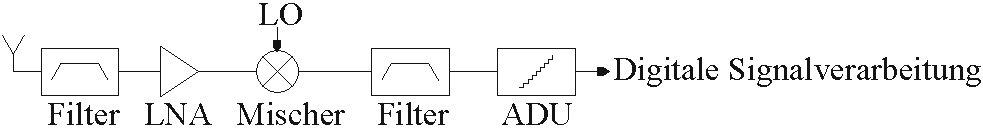
\includegraphics[width=14cm]{XX_DEMO_empfaenger} %Größe, Ort, am besten als vektorgraphik (pdf), Photos als jpg
\caption{Beschreibung (Quellen dahinter) \cite{BibDEMO1}\cite{BibDEMO2}}
\label{fig:textreferenz}
\end{figure}

Eine Quelle wird direkt hinter dem Satz vor dem Punkt angegeben mit \cite{BibDEMO1}, oder aber hinter einem kompletten Absatz. Auch Formeln (im Text) und Bilder (in der caption) müssen eine Quellenangabe enthalten.

Schöne Schaltpläne lassen sich auch direkt in Latex mi tikz/circuitikz malen, siehe \ref{tikz}.

\begin{figure}
	\centering
	\tikzsetnextfilename{XX_DEMO_tikz} %Dateiname, unter der die datei im ordner tikz-ext-out angelegt wird
	\tikzset{external/remake next} %uncomment to force remake figure
	\begin{tikzpicture}[scale=.8,transform shape]
	
	\draw  (0,0)coordinate[rground](start) to [vsourcesin,v<=$u_e$]++(0,3)to[R,l=$R_1$]++(4,0)coordinate[circ](knoten1)
			to [R,l=$R_3$]++(4,0) coordinate[circ](knoten2) --++(1,0) node[op amp,anchor=-](opv){};
			\draw (knoten1) to[C,l=$C_2$](knoten1|-start) coordinate[rground];
			\draw (knoten2) to[C,l=$C_1$]++(0,3) coordinate[circ](knoten3);
			\draw (knoten1) to[R,l=$R_2$]++(0,3)--(knoten3);
			\draw (opv.out)--++(1,0)|-(knoten3);
			\draw (opv.+)--++(-1,0)--++(0,-1)coordinate[rground];
			\draw (opv.out)++(1,0)to[short,*-o]++(1,0) coordinate(out);
			\draw  [->,shorten >=1ex,shorten <=1ex,thick] (out) -- (out|-start) node[left,midway] {\Large$u_a$};
			\draw (out|-start) coordinate[rground] coordinate[ocirc];
			
			\draw (knoten1) node[above left]{$\varphi_1$};
			\draw (knoten2) node[above left]{$\varphi_2$};
	\end{tikzpicture}
	\caption{Toller Schaltplan mit circuitikz (\url{https://github.com/lte-fau/circuitikz})}
	\label{tikz}
\end{figure}

\subsection{Formeln}

Auf Formeln kann mit \ref{eqn:tc} verwiesen werden. Konstanten und mathematische Funktionen (z.B. ln), sowie Einheiten sollten dabei nicht kursiv geschrieben werden. Zwischen einer Zahl und der Einheit ist ein halbes Leerzeichen mit 1,0\,\textmu V zu setzen. Das Komma ist bei der Zahl kein Punkt, die für Spannung steht das deutsche "`U"' und nicht "`V"'.

\begin{eqnarray}\label{eqn:tc}
X_{Strom}=\text{Konstante} \cdot 1,0\,\text{mV} \cdot \frac{1}{I} \cdot \frac{\partial I}{\partial T}
\end{eqnarray}

\subsection{Häufige Fehler}
Es sollten alle Dokumente im Format "utf8" gespeichert werden.

%Kommentare sind jederzeit mit einem %-Zeichen möglich	
	%\input{Abschnitte/Grundlagen}
	%\input{Abschnitte/Stand_der_Technik}
	%\input{Abschnitte/Entwurf}
	%\input{Abschnitte/Aufbau}
	%\input{Abschnitte/Messung}
	%\input{Abschnitte/Zusammenfassung}
	\chapter{Zusammenfassung und Ausblick}
\label{sec:Zusammenfassung}
\pagestyle{scrheadings}




Zur weiteren Verbesserung wäre noch das Eruieren des Grundes für den schlechten Empfang am Transceiver $3$ notwendig. So könnte durch das Anschließen eines Signalgenerators an die Antennenbuchse der entsprechenden Transceiverbaugruppe ein möglicher Fehler im Anpassnetzwerk aufgezeigt werden. Sollte auch dies nicht zu einer Verbesserung führen, wäre ein Austausch des \acp{IC} notwendig.
Für das bessere Erkennen von doppelten Übertragungen wäre das Einfügen eines Zeitstempel in die Ausgabe hilfreich. Dadurch könnten Übertragungen die kurz hintereinander eintreffen markiert und entsprechend zu einer korrekten zusammengefügt werden. Zu diesem Zweck würde es sich anbieten die Realtime-Clock des XMC4500 zu verweden. Dazu würde das auf der Platine vorsorglich verbaute Uhrenquarz verwendet werden. 


Auch wäre für eine Veränderung an der Platine die Auswahl eines anderen Eingangspins am XMC für das vom PP2 Pin des Transceiver 6 kommenden Interruptsignals sinnvoll. So wären die TDA3 und TDA6 nicht an den selben Interruptkanal des Mikrocontroller angeschlossen. Die dazu notwenigen Änderungen an der Software würden sich auf die Änderungen der entsprechenden Makros in der Headerdatei beschränken.
Alternativ ließe sich möglicherweise das Problem der konkurrierenden Interrupts über Anpassungen in der Software lösen. So wäre es möglich das Interruptsignal einzelner TDA5340 nicht über den PP2 Pin auszugeben, sonder auch über die ebenfalls mit dem XMC verbundenen PP0 und PP1 Pins. Somit wäre ein verteilen auf einzelne Kanäle der \ac{ERU} wahrscheinlich möglich.




	%\input{Abschnitte/Literaturverzeichnis}
	
	
	%Index (eigens hinzugefügt)
	\newpage
	\renewcommand{\indexname}{Stichwortverzeichnis}
	\printindex
	%index ende
	
	\listoffigures
	\listoftables
	\lstlistoflistings
	
	

	%\include{Abschnitte/Lebenslauf} 
	\chapter{Anhang}
\label{sec:Anhang}
\pagestyle{scrheadings}
EINFÜGEN:
Layout Stefan Erhard
Bilder Altium
3D Modelle


\section{Seriennummern}
\label{app:Seriennummern}
Alle TDA5340 verfügen über eine eingebaute Seriennummer, welche ausgelesen werden kann. Die Seriennummern der verwendeten TDA5340 sind in der Tabelle aufgeführt.
\begin{table}[h]
\centering
\begin{tabular}{cc}
TDA & Seriennummer\\
\hline
TDA1 & 33020236\\
TDA2 & 11727080\\
TDA3& 11545236\\
TDA4& 11728870\\
TDA5& 11550773\\
TDA6& 33026263\\
\end{tabular}
\caption{Seriennummern der im Projekt verwendeten TDA5340 }
\label{default}
\end{table}%

\section{3D-Daten}
\subsection{Gehäuse}
\label{app:Gehäuse}
 
	
	\chapter*{Literatur}
	\printbibliography[heading=none]
\end{document}